\documentclass{article}
\usepackage{amsmath}
\usepackage{mathtools}
\usepackage{txfonts}
\usepackage[margin=0.5in]{geometry}
\usepackage{graphicx}
\usepackage{float}
\usepackage{booktabs}
\usepackage[caption=false]{subfig}
\graphicspath{ {images/} }
\usepackage{appendix}
\usepackage{url}



\setlength{\parskip}{\baselineskip}%
\setlength{\parindent}{0pt}%

\title{A regression model for predicting rail transit ridership at the station level}
\author{Daniel Hartig}
\date{\vspace{-5ex}}


\begin{document}
\maketitle

\section{Introduction}

The United States is undergoing a rail boom. Since 2010, new light rail lines have opened in Dallas, Los Angeles, Salt Lake City, Denver, Minneapolis, Houston, Seattle and more.  A new heavy rail line opened in Washington DC, and a commuter rail system in Orlando. As transit expands in cities in the United States, there is an opportunity to validate predictive rail ridership models. 

A survey of transit agencies \cite{Boyle2006} conducted by the Transit Cooperative Research Program showed that relatively few agencies are using quantitative models when forecasting ridership for new lines, extensions or stations under consideration for funding. Of the 35 agencies that responded to the survey, 29 use professional judgment and 28 use rules of thumb among one or more techniques used to generate ridership forecasts. Another method used by 22 agencies is service elasticity; a set of general transit demand response curves for changing transportation options, published by the Transportation Reserach Board \cite{tcrp95}. 

For quantitative methods, the most commonly used technique--by 18 of 35 surveyed agencies--is the four-step travel demand model \cite{McNally2008}, introduced by Mannheim and Florian \cite{Mannheim1979, Florian1988}. The Mannheim-Florian model's four steps are trip generation, trip distribution, mode choice and route choice. In the trip generation phase, trip endpoints are created with as production and attraction ends. In the trip distribution step, these endpoints are paired up to generate trips; for example a residence with a a job, or hotel with a tourist attraction. In the mode choice step, trips are assigned to various transportation modes, such as personal vehicle, bus, or walking. Finally, in the route choice step, a route using that mode of transportation is chosen.

An implementation of the Mannheim-Florian model can be seen in the Seattle's Sound Transit Ridership Forecasting Methodology Report \cite{ST3_2015, ST3_add}. The Sound Transit 3 (ST3) was a ballot measure that passed in 2016 for a \$54 billion expansion of the local light rail system involving 100 km of new tracks and 37 new stations. The ridership forecasting methodology report explained how the project's official ridership projections were developed. The regional area is divided into 785 Alternatives Analysis Zones and for each of these zones transit surveys and recorded ridership on local bus routes were used to complete the trip generation and trip distribution steps. The mode choice and route choice is done using an incremental logit model to predict changes in transit mode based on changes in transit mode availability.

Only seven of the 35 surveyed agencies used regression models among the methods to predict future transit ridership. This thesis proposes a regression-based model based on data from the United States Census Bureau at the zip code level. The model will be trained on the zip code characteristics and ridership data from existing light and heavy rail transit systems and used to predict ridership on other rail transit systems.  

The Mannheim-Florian four step model fundamentally depends on already existing transit information. For example, the starting point of a four step analysis for a new light rail line would be an existing bus line that runs a similar, hopefully identical, path. The advantage of a regression model is that it creates a new estimate from different sources. Even if a regression model's accuracy is not superior to that of a four step model used on the same transit network, the regression model is still valuable because it produces a second, independent quantitative estimate. This estimate can be used to validate or adjust any existing model. 


\section{Data and Methodology}

\subsection{Data Sources for Predictor Variables}

The zip code level data for feature generation comes from the US Census Bureau and is available at \texttt{factfinder.census.gov}. There are thousands of potential data sets available. Selection of features is guided by Kuby \cite{Kuby2004}, Taylor \cite{Taylor2008}, and Currie \cite{Currie2011}, which demonstrate the significance of factors such as employment, population, universities, poverty, airports, park and ride stations, and rental units. In Yao \cite{Yao2007}, a distinction is made between `Need Index,' a series of features that depend on the characteristics around the station and are independent of the transit network, and transit network characteristics, which do depend on the transit network. To model network characteristics for each station, the sum of each characteristic for every other station within 15 and 30 minutes transit time is included as a feature of the original station. This also provides us quantitative way to express the 'centrality' dummy variable that is provided as a flag in many models \cite{Kuby2004, Durning2015}; centrality could be proportional to the count of population or jobs within 30 minutes of a station, for example.

This model emphasizes using only feature that have 'real' units. Only a single feature (presence of a park and ride garage) is a flag. Instead of using measures of land use mix as proposed in other models \cite{Durning2015, Gutierrez2011}, or dummy variables for universities and central business districts, the equivalent information is provided naturally as counting data in the feature set. Housing types (such as large apartment buildings versus single family homes) can stand in for land use mix, number of jobs at universities or in financial jobs can file in for the equivalent dummy variable. A summary of the selected characteristics is provided in Appendix \ref{app:features}.

Ridership data for agencies that publish annual ridership reports is used to validate the model (see Appendix \ref{app:ridership}). Six cities were selected for this study: Boston, Chicago, Los Angeles, Atlanta, Dallas, and Denver. Several cities were eliminated from the sample set for various reasons. The Census Bureau data set does not include government employment. While state level employment is significant in all potential cities, state employment levels are relatively constant from city to city. Federal employment varies greatly, however. Washington DC was eliminated due to the large impact of un-recorded federal employment. San Francisco and Philadelphia were eliminated because they have multiple rail systems without integrated fares. New York City was eliminated because it's subway has higher ridership than all other rail systems in the country combined. 

The data closest to 2015 is used when possible to get an accurate relation between ridership and census data. The census data as well as Chicago, Dallas, Denver's ridership statistics are from 2015. Boston's ridership is from 2014, Los Angeles' is from 2013-2014, and Atlanta's is from 2010-2013. 



\subsection{Feature Generation}

We translate zip code level data into transit station specific data by sampling each zip code's geographic area to determine proximity to a transit station. For each zip code near the transit network, a set of random points within that zip code is generated using rejection sampling. For each of the those points, the one or more closest stations are determined. Each point is assigned to one or more station within walking distance. Counts for the characteristics of each zip code, such as population or employment, are then assigned to each station proportional to the number of points assigned to each station.

\subsubsection{Rejection Sampling of Zip Code Shapefiles}

The US Census Bureau provides TIGER/Line shapefiles of each zip code tabulation area (ZCTA) in the United States at \linebreak\texttt{https://www.census.gov/geo/maps-data/data/tiger-line.html}.  From a box drawn around the extremities of each zipcode's shape, random points are accepted if they are within the shapefile or rejected if they are outside it. Those points that are inside the shapefile are tested against author-created exclusion zones. These zones are shapes within the zip code's shapefile area that are known to not have any population, employment, or other countable characteristics. The exclusion zones are mostly drawn over water areas, or large parks. Those points that are inside the exclusion zones are also rejected.

The remaining points are tested for their distance to any transit stations. The area within walking distance of a station is its catchment. A standard transit catchment distance for rail is one half mile (800 m), although Guerra \cite{Guerra2012} suggests that one half mile is more appropriate for population as a feature while one quarter mile (400 m) is better for employment. A case study \cite{ElGeneidy2014} from a 2003 Montreal transit riders origin-destination survey concluded that approximately 50\% of riders of the city's urban rail transit walk less than 500 meters to their stations, while 90\% walk less than 1000 meters. The maximum walking distance is approximately 1500 meters. Another analysis \cite{Gutierrez2011} found the optimal distance for  for assigning population and employment to a station was between 600 and 900 meters in straight line distance, with no distance weighted decay. 

Given this information, we choose cutoffs of 500 meters and 1000 meters for calculating station distances. Each tested point is divided between all stations within 500 meters. If there are no stations within 500 meters, then the point is divided between all stations within 1000 meters. If no stations are within 1000 meters, that point is not assigned to any station. The total sum of points and fractional points assigned to each station is divided by the total points available. The station's portion of each of the zip code's characteristic data counts is assigned to that transit station. 

\begin{figure}[H]
\begin{center}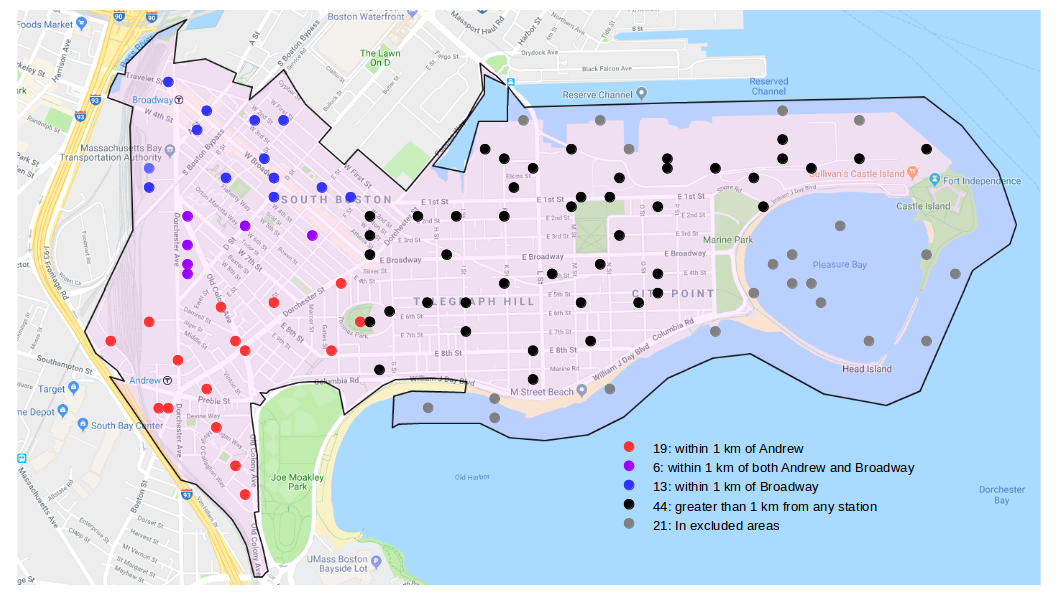
\includegraphics[scale=0.6]{geo_point_demonstration}\end{center}\caption{Illustration of nearest zip code estimation for zip code 02127.}\label{fig:f1}
\end{figure}


An example using zip code 02127, the South Boston neighborhood of Boston, illustrates the sampling method (Figure \ref{fig:f1}). 100 random points are selected within the area of the shapefile. Of these, 21 are rejected due to exclusion areas based on water area, parks and abandoned port facilities. Of the remaining 79 points, 8 are within 500 meters of Andrew station, while 6 are within 500 meters of Broadway station. Moving out to the 1000 meter radius, 11 are within 1 km of Andrew station, for a total of 19 closest to Andrew; 7 are within 1 km of Broadway station for a total of 13 closest to Broadway; and 6 are within 1 km of both. The 6 stations within 1 km of both stations are divided between the two. The total population of South Boston is 36494. Therefore, $$\frac{19 + \frac{6}{2}}{79}\cdot{36494} = 10163$$ people are assigned to Andrew station. Similarly, 7391 people are assigned to Broadway station. This calculation is performed for all countable features and all zip codes and summed total counts for each characteristic are used as a feature for each transit station. 

\subsubsection{Generation of network-dependent features}

For each `Need Index' type feature generated by rejection sampling, a set of corresponding network-based features are generated to represent the sum total of a certain characteristic (such as population or employment) within a given travel time of that station. The transit network is laid out as a graph, where nodes represent the transit stations and edges are weighted to the travel time between the stations, according to the website of the transit agency. At transfer points, there is a separate node for a single station on each line. The edge between these two nodes is the average wait time for transfer between the trains. 

An illustration of the calculation of travel time between Sullivan Square and South Station in Boston is provided in Figure \ref{fig:f2}. Starting at Sullivan Square on the Orange Line southbound, there are four edge traversals totaling seven minutes to get to Downtown Crossing. From there, there is a 2.5 minute wait until a Red Line (also Southbound) train arrives, and 2.5 more minutes of travel to South Station. The total travel time is thus twelve minutes. 

\begin{figure}[H]
\begin{center}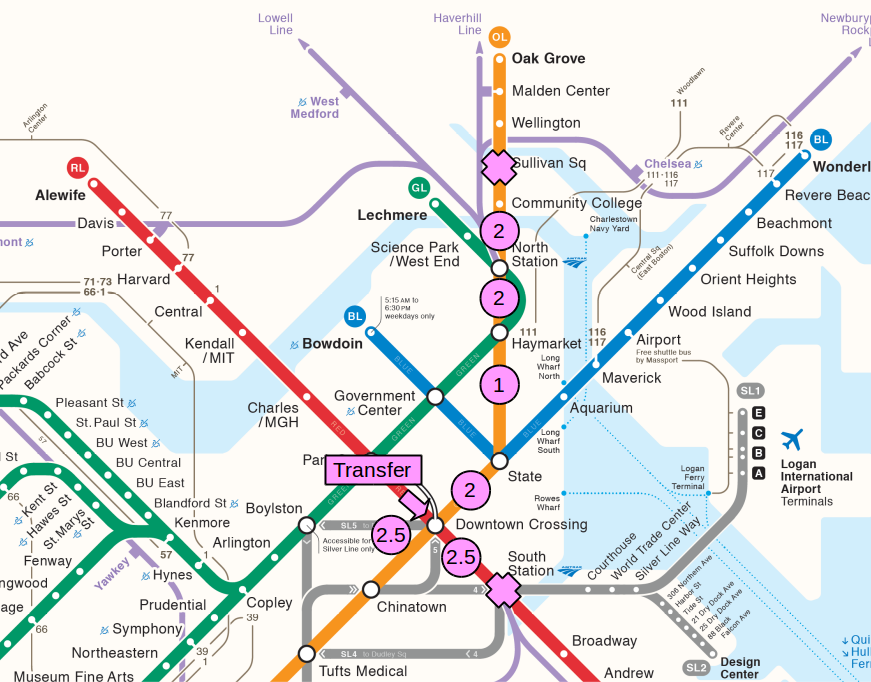
\includegraphics[scale=0.75]{transfer_demonstration}\end{center}\caption{Illustration of travel time calculation for Sullivan Square to South Station, in Boston.}\label{fig:f2}
\end{figure}

\subsection{Metrics for projection accuracy assessment}

In general, the projected ridership forecasts of new transit infrastructure investments significantly overestimates transit ridership. The pioneering study in this field by Pickrell in 1989 \cite{Pickrell1989} found that for ten rail projects completed between 1977 and 1985, and assessed between 1986 and 1989, the actual ridership was between 28\% and 85\% lower than projected. A 2006 study \cite{Flyvbjerg2006} of 25 major passenger rail projects in  in 14 nations found that 21 of the projects had actual ridership below projections, with the average system ridership 48\% below the projection. Accurate assessment of projection accuracy is imperative for creating ridership estimates that serve the public interest.

To assess the results of regression analysis, there should be two metrics used: one for the total system level ridership, and another for station level ridership. Following Pickrell, the metric for system-wide projection accuracy is standard percentage error in total system ridership, which we will refer to as system error. Hardy \cite{Hardy2010} extends Pickrell's analysis by including absolute station error for stations on newly added sections of an existing transit network. Following Hardy, a measure of station level error on a network is summed absolute error of all station projections. The rail networks in this study vary widely in total ridership; therefore, to allow network to network comparison, this summed absolute station error can divided by total system ridership. The resulting metric for station error given a projected ($y_{proj}$) and actual ridership ($y_{true}$) is 
$$SSE = \dfrac{\sum\limits_{i\,\in\,\text{all station}}\left|y_{proj, i} - y_{true, i}\right|}{\sum\limits_{i\,\in\,\text{all station}} y_{true, i}}$$






\begin{figure}
\centering
\begin{minipage}{0.5\textwidth}
\centering
\subfloat[Ridership against population. Linear regression in red, log regression in blue.]{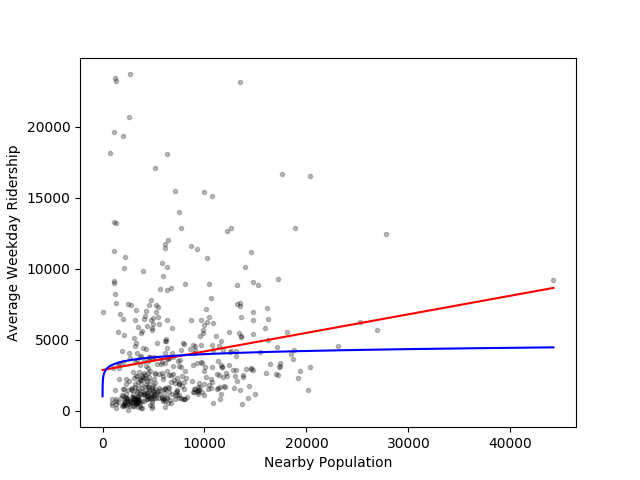
\includegraphics[clip,width=\columnwidth]{popvrider}}

\subfloat[Residual from linear regression against population]{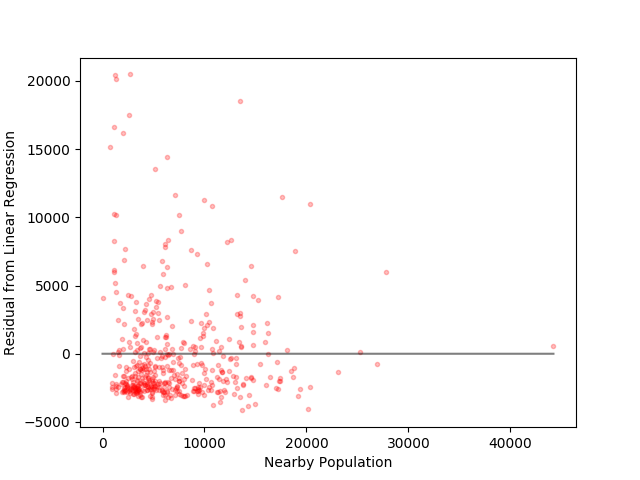
\includegraphics[clip,width=\columnwidth]{poplinresid}}

\subfloat[Residual from log regression against population]{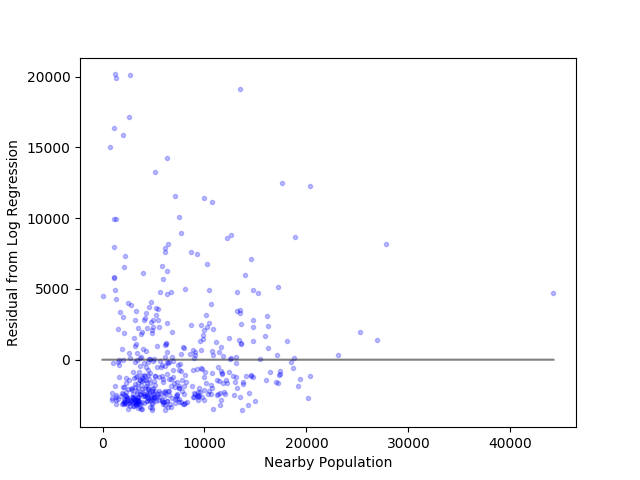
\includegraphics[clip,width=\columnwidth]{poplogresid}}
\caption{Analysis of population regression}\label{fig:popresid}
\end{minipage}\hfill
\begin{minipage}{0.5\textwidth}
\centering
\subfloat[Ridership against employment. Linear regression in red, log regression in blue.]{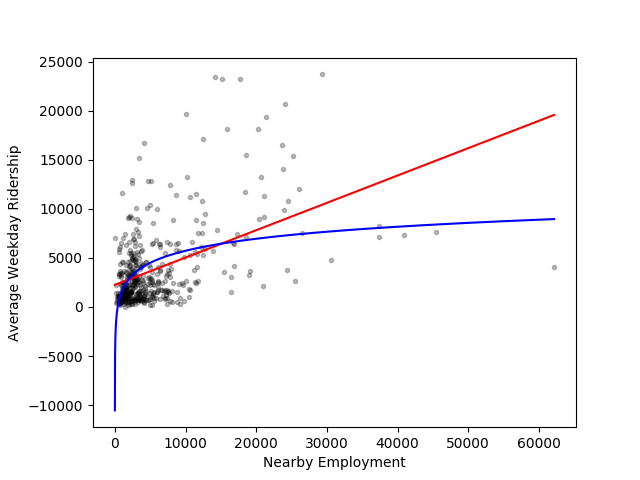
\includegraphics[clip,width=\columnwidth]{empvrider}}

\subfloat[Residual from linear regression against employment]{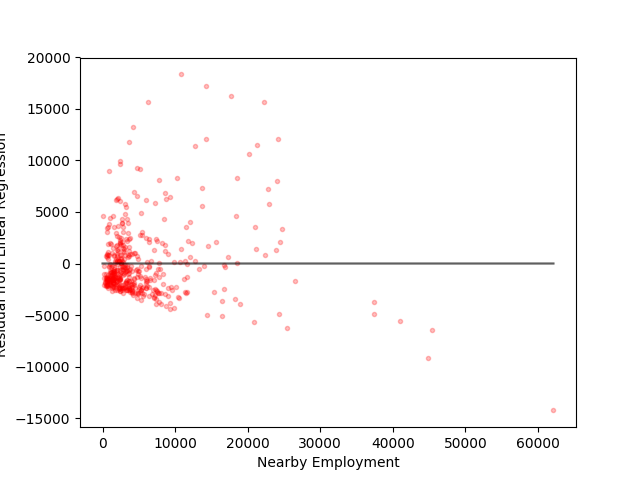
\includegraphics[clip,width=\columnwidth]{emplinresid}}

\subfloat[Residual from log regression against employment]{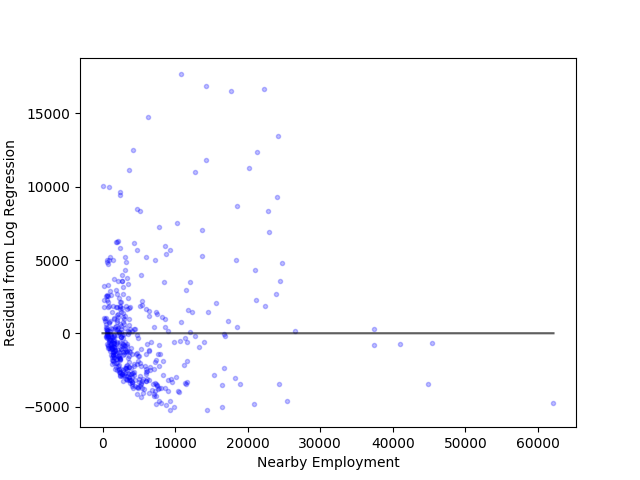
\includegraphics[clip,width=\columnwidth]{emplogresid}}
\caption{Analysis of employment regression}\label{fig:empresid}
\end{minipage}\hfill
\end{figure}

\subsection{Regression Analysis}

Regression models for station level ridership have used ordinary least squares regression \cite{Kuby2004, Taylor2008, Currie2011, Durning2015, Gutierrez2011} to generate predictions. We will investigate the applicability of more complex regression models.

\subsubsection{Data distribution and regression selection}
There are generally two types of feature included in this survey, those that are related to population and those that are related to employment. Features such as the population with college degrees and number of housing units will be related to population. Features such as the number of jobs in finance or hospitality will be related to the total number of jobs. A plot of all stations' population versus ridership appears in Figure \ref{fig:popresid} with linear and logarithmic regression lines and residuals. A similar treatment for employment versus ridership appears in Figure \ref{fig:empresid}. The coefficient of determination for the two regression types for both population and employment are shown in Table \ref{tab:regr2}.

\begin{table}[H]\label{tab:regr2}
\centering
\begin{tabular}{lcc}
\toprule Variable&Linear R$^2$&Log R$^2$ \\ 
\midrule Population&0.0267&0.0034 \\
Employment&0.1948&0.1878 \\
\bottomrule
\end{tabular}
\caption{Regression of Population and Employment against ridership}
\end{table}

The metrics for projection accuracy depend on the absolute difference between actual and predicted ridership. This suggest that Least Absolute Deviations (LAD) regression is appropriate for this problem. 

Since the response variable (ridership) is counts, and the variance of ridership increases with increasing employment, we will also use Poisson regression. As demonstrated in Table \ref{tab:regr2}, there does not appear to be any modeling advantage of using a logarithmic form of the feature variables. The log link also causes problem with outliers when the regression model is cross validated, so we use the identity link with Poisson regression instead of the canonical log link. 

Finally, we will use ordinary least squares (OLS) regression as a comparison, to see if the other methods have any performance advantage. 

\subsubsection{Feature selection by LASSO regularization}

Upon performing regression analysis, it became immediately apparent that one set of features was different from the others. The number of students within a 15 or 30 minute transit trip proved to be a very accurate measurement of system level ridership. These variable are represented in the model as \texttt{15net\_students} and \texttt{30net\_students}, respectively. We show the results of a single variable OLS regression of the one variable against ridership. The scores are the average of the six way cross-validation across the six transit networks in the study. The `best' scoring other feature (\texttt{15net\_hunits\_old}; the number of housing units built before 1940 within a 15 minute transit ride) is shown for comparison.

\begin{table}[H]\label{tab:students}
\centering
\begin{tabular}{lcc}
\toprule Variable&System Error&Station Error\\
\midrule 30net\_students&0.1016&0.5961\\
15net\_students&0.0946&0.6197\\
15net\_hunits\_old&0.2854&0.6700\\ 
\bottomrule
\end{tabular}
\end{table}

The system error scores for \texttt{30net\_students} and \texttt{15net\_students} are much lower than for any other variable, while the station error for these features are also lower than any other features. As we will see, the single-feature OLS of either of these features produces a model that is approximately as good as any other model we will develop. This raises questions about the relationship between the feature and the response variable. It is possible that the population of students within walking distance of a transit station is driven by the availability of local transit. In that case, number of students is not a valid explanatory variable. Since the relationship is unclear, but the features are outliers, we will remove all features derived from number of students from the model.



 

The following chart (Table \ref{tab:lasso}) shows the results for the three regression types. 





\subsubsection{Feature selection by brute force}

The brute force method is a greedy search of all possible features to find the best 'path' to a regression solution. First, all features are checked by regression against ridership. Since we have two 'score' metrics, we use the average of system and station error to determine the best feature in each step. Each feature is checked in six-way cross validation. Each of the six cities is used as the test set while the other five are used for the training set. The average over all six cross-validation runs for each metric is what is reported in the charts below. 

After choosing the one feature that yields the highest score, we then select a second feature to add to the regression in in the same way, and iteratively add more features. The subsequent steps are multiple regressions using all of the already chosen features. 

We select the fist 25 features with this method and graph the resulting system and station error scores in Figure \ref{fig:bfscores}. 

\section{Conclusion and further work}


\pagebreak
\begin{appendices}

\section{Data sources}

\subsection{Ridership data}\label{app:ridership}
\begin{tabular}{ll}
Los Angeles: & \url{http://libraryarchives.metro.net/DPGTL/Ridership/RailActivityByStationFY2014.xls} \\
Chicago:& \url{http://www.transitchicago.com/assets/1/ridership_reports/2015_Annual.pdf} \\
Atlanta:& \url{http://documents.atlantaregional.com/transportation/TFB_2014_v17.pdf}\\
Boston:& \url{http://archives.lib.state.ma.us/bitstream/handle/2452/266319/ocm18709282-2014.pdf} \\
Denver:& \url{http://www.rtd-denver.com/documents/serviced/lrt-activity-08-2015.pdf} and \\
& \url{http://www.rtd-denver.com/documents/serviced/lrt-activity-Jan-April-2016.pdf}\\
Dallas:& \url{https://www.dart.org/about/dartreferencebookmar16.pdf}\\
\end{tabular}

\subsection{US Census feature data sources}\label{app:features}

All feature data is accessed through the American Factfinder website at \url{factfinder.census.gov}.

\begin{tabular}{ll}
Population&Table DP05, Item HC01\_VC03\\
Population, 18 and under&Table DP05, Item HC01\_VC03 - Item HC01\_VC32\\
Population, 65 and over&Table DP05, Item HC01\_VC37\\
Housholds&Table S1101, Item HC01\_EST\_VC02\\
Households with Children&Table S1101, Item HC01\_EST\_VC06\\
Families&Table S1101, Item HC01\_EST\_VC010\\
Population with at least Bachelors degree&Table S1701, Item HC01\_EST\_VC34\\
Population in labor force&Table S1701, Item HC01\_EST\_VC37\\
Employed population&Table S1701, Item HC01\_EST\_VC38\\
Full-time employed population&Table S1701, Item HC01\_EST\_VC47\\
Population living at greater than 500\% of poverty level&Table S1701, Item HC01\_EST\_VC56\\
Population living at less than 200\% of poverty level&Table S1701, Item HC01\_EST\_VC01 -  HC01\_EST\_VC59\\
Housing units&Table DP04, Item HC01\_VC03\\
Single-family detached housing units&Table DP04, Item HC01\_VC14\\
Housing units in duplexes or townhouses&Table DP04, Items HC01\_VC15 + HC01\_VC16\\
Housing units in structures of 3-9&Table DP04, Item HC01\_VC17 + HC01\_VC18\\
Housing units in structures of 10+&Table DP04, Item HC01\_VC19 + HC01\_VC20\\
Housing units built before 1940&Table DP04, Item HC01\_VC36\\
Housing units built after 2000&Table DP04, Item HC01\_VC27 + HC01\_VC28 + HC01\_VC29\\
Housing units occupied by owner&Table DP04, Item HC01\_VC65\\
Housing units occupied by renter&Table DP66\\
Number of Jobs&Table CB1500CZ11, Item ‘EMP’\\
Total pay of all jobs&Table CB1500CZ11, Item ‘PAYANN’\\
Number of jobs at hospitals&Table CB1500CZ21, NAICS code 622, Estimated\\
Number of jobs at universities&Table CB1500CZ21, NAICS code 6113, Estimated\\
Number of jobs in hospitalitiy field&Table CB1500CZ21, NAICS code 72, Estimated\\
Number of jobs in finance field&Table CB1500CZ21, NAICS code 52, Estimated\\
Number of jobs in professional fields&Table CB1500CZ21, NAICS code 54, Estimated\\
Number of jobs in entertainment fields&Table CB1500CZ21, NAICS code 71, Estimated\\
\end{tabular}




\section{Summary of selected features}

For the brute force results, the best one feature is selected by six way cross validation for each step, from one to twenty five. For the LASSO feature selection, each of the six cross-validated models produces a unique set of features. Therefore, each feature is selected up to six times. Those features selected by at least four of six crass validated runs are marked on the table below. For the LAD LASSO, the number of features selected by LASSO is unusually high, so those features selected by at least five of size cross validated runs are selected, to avoid saturated models. 

\begin{tabular}{lcccccc}





\end{appendices}










 
\bibliographystyle{unsrt}
\pagebreak\bibliography{bibrefs}





\end{document}